\section{Introduction}
\label{section:introduction}
At the basis of this study we aim to express the potential of using number of robotic arms in parallel. Despite the usage of robotic arms in large applications at the industry (especially in the automotive industry) in most cases they are operating as separated units. As shown in figure \ref{fig:automotive_industry_example} a car assembly line is built by a large number of robotic arms where some arms are sharing their workspaces. To avoid collision between a couple of arms a coordination method is applied, this method is based on timing principles such that the motions are priorly calculated. This means that the assembly line runs on open loop and any small changes of the sequence can cause a crush. On the contrary, having an autonomous method for coordinating motions that is based on the current state of the system may affect 3 aspects that directly connected to manufacturing costs:

\begin{enumerate}
\item The total time spent on manufacture a single vehicle may reduce.
\item The assembly line size may decrease.
\item A single assembly line can handle many models of vehicles.
\end{enumerate}



\begin{figure}[htb]
\centering
\begin{subfigure}{.5\textwidth}
  \centering
  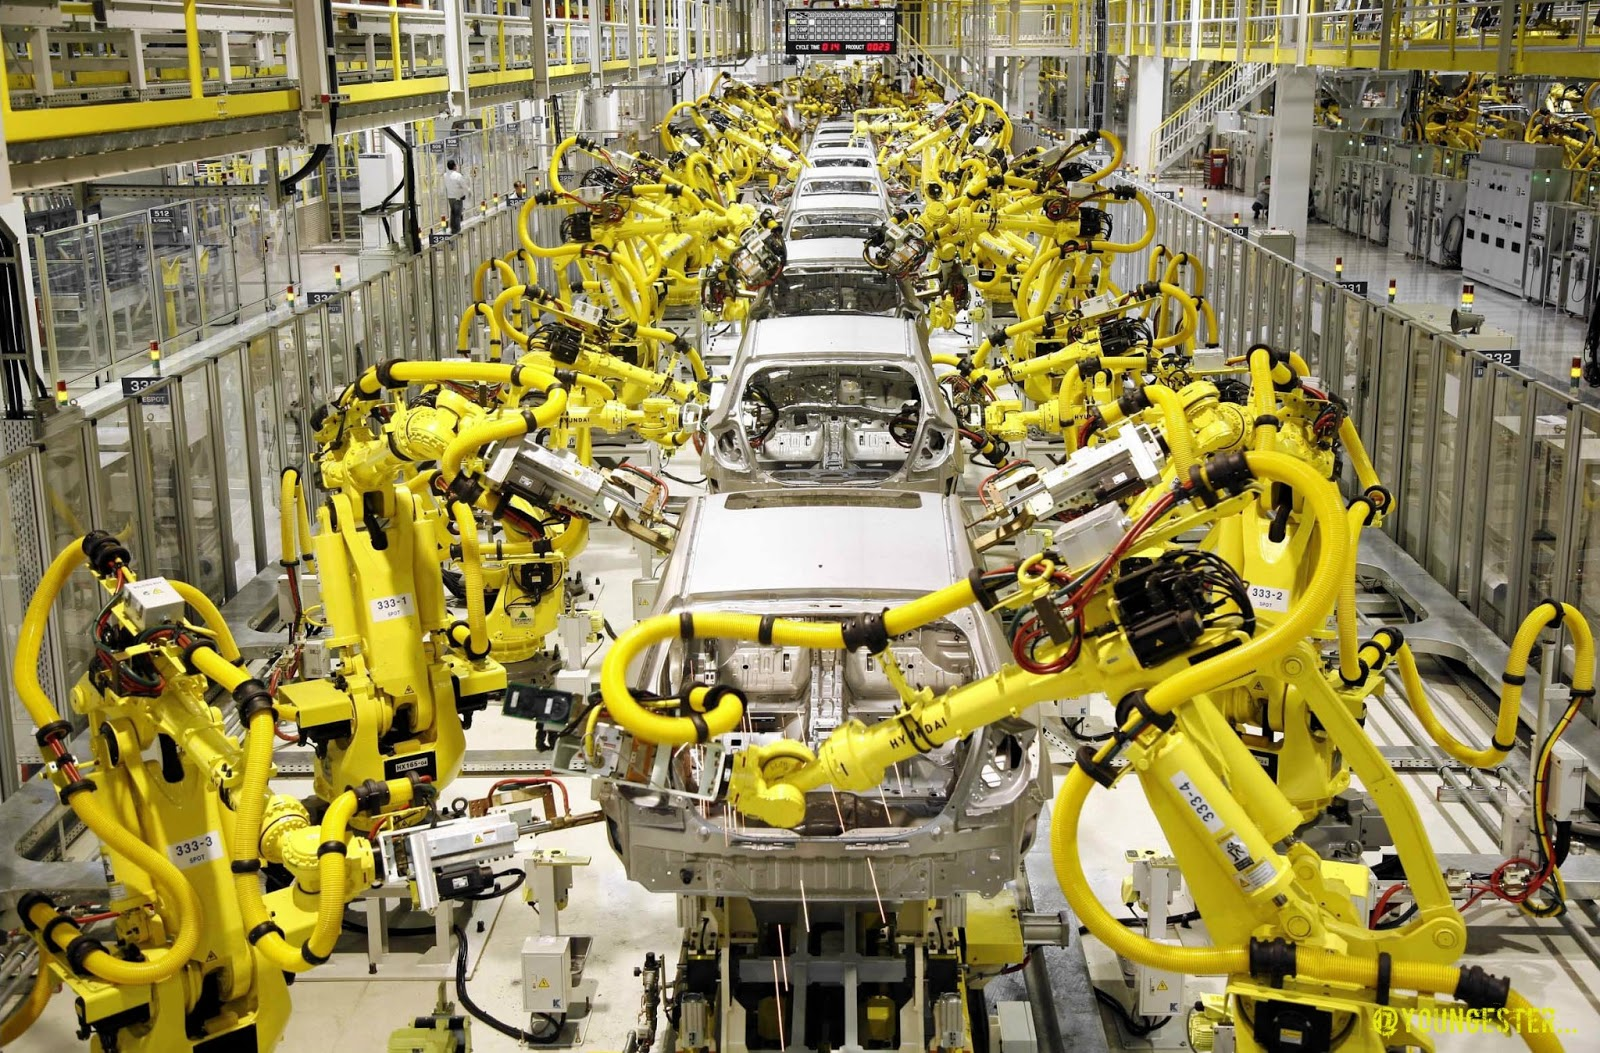
\includegraphics[scale=0.3,width=\textwidth]{Industry}
\end{subfigure}%
\begin{subfigure}{.5\textwidth}
  \centering
  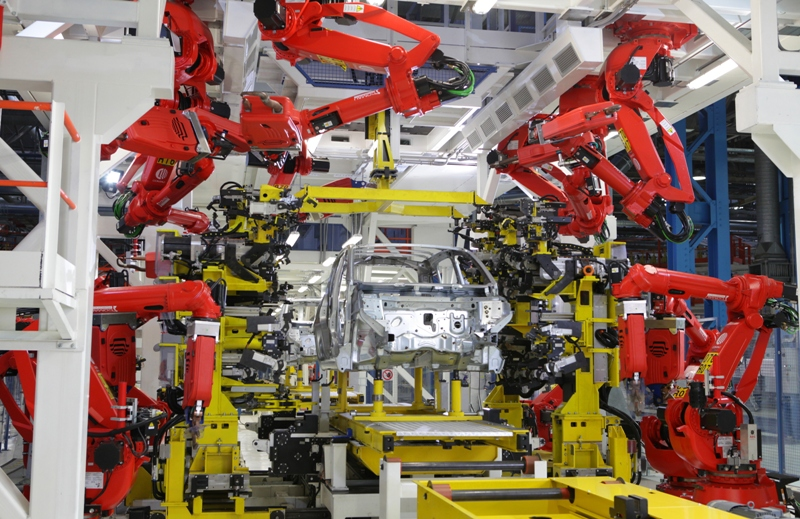
\includegraphics[scale=0.3,width=\textwidth]{Industry2}
\end{subfigure}
\caption{Assembly lines in the automotive industry}
\label{fig:automotive_industry_example}
\end{figure}
